\section{Parameters}

\begin{figure}
    \centering
    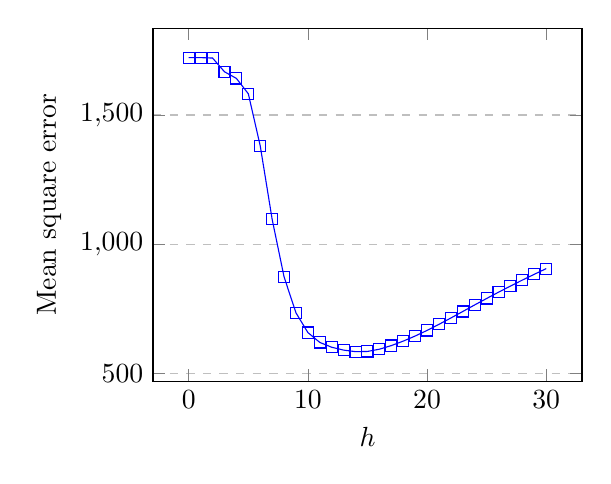
\begin{tikzpicture}
        \begin{axis}[
            title={},
            width=20em,
            xlabel={$h$},
            ylabel={Mean square error},
            legend pos=north west,
            ymajorgrids=true,
            grid style=dashed,
        ]
         
            \addplot[
                color=blue,
                mark=square,
                ]
                coordinates {
                    (0, 1722.1568944359642)
                    (1, 1722.1568944359642)
                    (2, 1720.5348812267416)
                    (3, 1667.4070565582194)
                    (4, 1641.6590045194696)
                    (5, 1582.3359946325063)
                    (6, 1380.382551155807)
                    (7, 1096.2059775722566)
                    (8, 873.4298110402761)
                    (9, 734.1602815440025)
                    (10, 657.990290124011)
                    (11, 619.8022931569443)
                    (12, 601.14668073389)
                    (13, 590.0937914658845)
                    (14, 584.0679840970539)
                    (15, 584.927498927499)
                    (16, 593.6357287520078)
                    (17, 607.6320797541728)
                    (18, 624.907557890116)
                    (19, 644.5614094160605)
                    (20, 666.2656635040356)
                    (21, 689.8439535881396)
                    (22, 714.4187268664012)
                    (23, 739.6025909630561)
                    (24, 765.0798414693763)
                    (25, 789.9337743058674)
                    (26, 814.3341564155518)
                    (27, 838.0244729779613)
                    (28, 861.2544072311514)
                    (29, 883.5748505981064)
                    (30, 905.4892525415781)
                };
        \end{axis}
    \end{tikzpicture}
    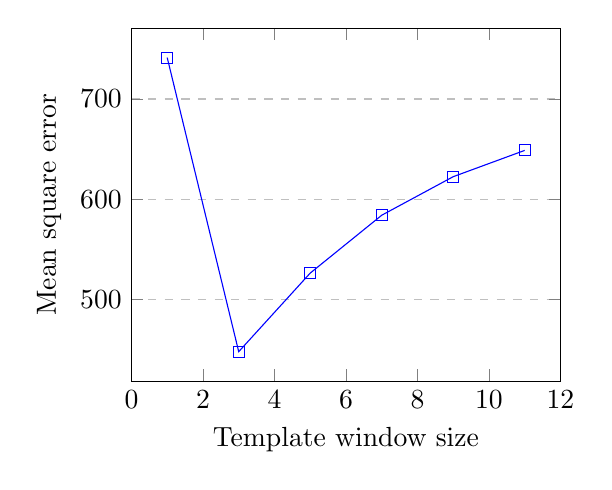
\begin{tikzpicture}
        \begin{axis}[
            title={},
            width=20em,
            xlabel={Template window size},
            ylabel={Mean square error},
            legend pos=north west,
            ymajorgrids=true,
            grid style=dashed,
        ]

            \addplot[
                color=blue,
                mark=square,
                ]
                coordinates {
                    (1, 741.2841579120649)
                    (3, 447.98107160316465)
                    (5, 526.3609614597987)
                    (7, 584.0679840970539)
                    (9, 622.5216894635499)
                    (11, 648.742619696108)
                };
        \end{axis}
    \end{tikzpicture}
    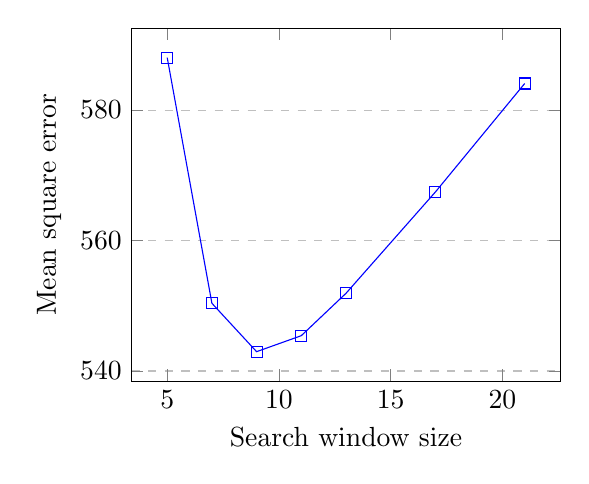
\begin{tikzpicture}
        \begin{axis}[
            title={},
            width=20em,
            xlabel={Search window size},
            ylabel={Mean square error},
            legend pos=north west,
            ymajorgrids=true,
            grid style=dashed,
        ]           
                    
            \addplot[
                color=blue,
                mark=square,
                ]
                coordinates {
                    (5, 588.0351306455958)
                    (7, 550.3852573503736)
                    (9, 542.9683013578363)
                    (11, 545.4179960691589)
                    (13, 551.9038390550019)
                    (17, 567.4274839623677)
                    (21, 584.0679840970539)
                };
        \end{axis}
    \end{tikzpicture}
    \caption{A graph showing how the mean square error is affected by the filter strength, template window size, and the search window size for a stock image.}
    \label{fig:mse}
\end{figure}

The filter strength $h$ is shown in Equation \ref{equ:f}.
Figure \ref{fig:mse} shows how the mean squared error 
(as in Definition \ref{def:mean-squared-error})
changes with this parameter $h$ for a stock image. It is shown that an increase in $h$ works
until a certain point (around $h = 14$) then becomes worse for values above that.
It is known that larger values of $h$ will remove noise \emph{better},
but also removes details from the image \cite{opencv} 
(this source also suggests a $h$ value of around 10).

It has been shown that locally calculating $h$ can be more beneficial then setting a global $h$ value;
using locally calculated $h$ values helps overcome a \emph{rare patch effect} 
shortcoming in non-local means \cite{duval2010parameter}.

A similar scenario can be seen for the template window size and the search window size
(see Figure \ref{fig:mse});
there is a value in which the algorithm performs best, and lower or higher makes it worse
